\documentclass[10pt]{article}
\usepackage{fontspec}
\usepackage{polyglossia}
\setdefaultlanguage{french}
\usepackage[a4paper,margin=2.5cm]{geometry}
\usepackage{url,hyperref}
\usepackage{siunitx}
\usepackage{schemabloc}
\usepackage{listings}
\usepackage{auto-pst-pdf}
\usepackage{pst-circ}
\usepackage{soul}
\usepackage{verbatim}
\usepackage{lmodern}
\usepackage{tikz}
\usepackage[european,cuteinductors,siunitx]{circuitikz}
\usepackage{xunicode,xltxtra}
\usepackage{graphicx}
\usepackage{amsmath}
\usepackage{minted}
\usepackage{multicol}
\title{
\includegraphics{../../../../images/inp-enseeiht} \\ ~ \\ ~ \\ ~ \\ ~ \\ Exercices de Matlab \\ Première séance : mode interactif }
\author{Guilhem Saurel}
\date{\today}
\renewcommand{\thesubsection}{\thesection .\Alph{subsection}}
\begin{document}

 \begin{titlepage}
  \maketitle
  \tableofcontents
 \end{titlepage}

 \section{Résolution d’une équation de second degré}
 
  \inputminted[linenos,firstnumber=1,firstline=1,lastline=2]{matlab}{un.m}
  \subsection{Utilisation de la méthode classique avec discriminant}
   \inputminted[linenos,firstnumber=3,firstline=3,lastline=6]{matlab}{un.m}
  \subsection{Utilisation de la fonction « root »}
   \inputminted[linenos,firstnumber=7,firstline=9,lastline=9]{matlab}{un.m}

 \section{Évaluation d’une fonction sur un intervalle}
  \subsection{}
   \inputminted[linenos,firstnumber=10,firstline=10,lastline=13]{matlab}{un.m}
   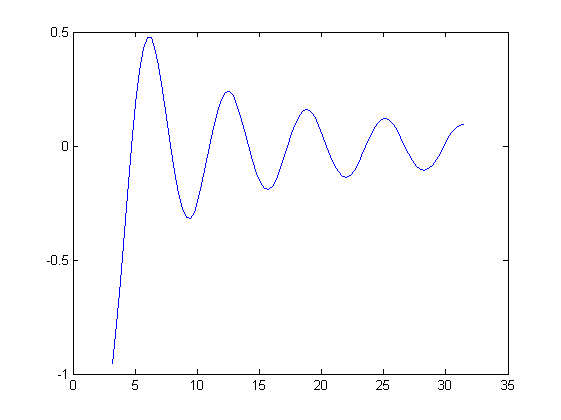
\includegraphics[width=5cm]{2A}
  \subsection{}
   \inputminted[linenos,firstnumber=14,firstline=14,lastline=17]{matlab}{un.m}
   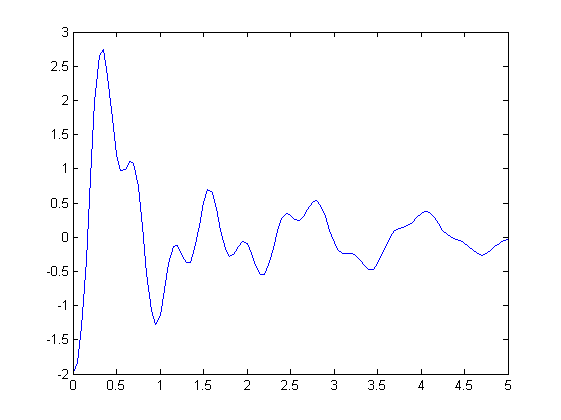
\includegraphics[width=5cm]{2B}
  \subsection{}
   \inputminted[linenos,firstnumber=18,firstline=18,lastline=21]{matlab}{un.m}
   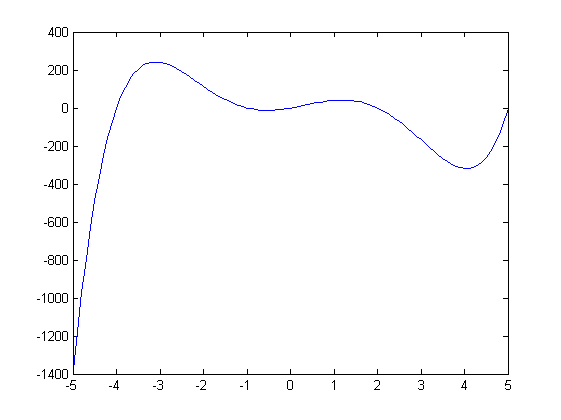
\includegraphics[width=5cm]{2C}
  \subsection{}
   \inputminted[linenos,firstnumber=22,firstline=22,lastline=28]{matlab}{un.m}
   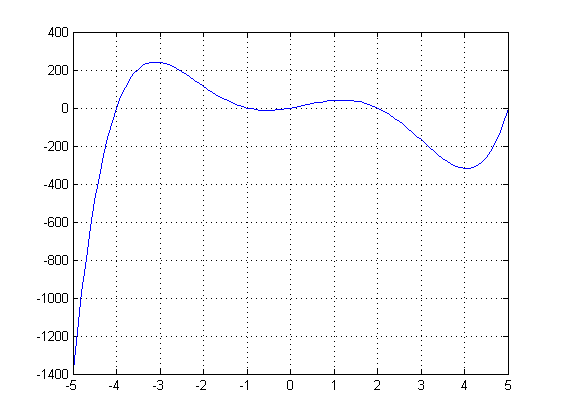
\includegraphics[width=5cm]{2D}

 \section{Calculs statistiques sur un ensemble de nombres}
  \inputminted[linenos,firstnumber=29,firstline=29,lastline=31]{matlab}{un.m}
  \subsection{}
   \inputminted[linenos,firstnumber=32,firstline=32,lastline=33]{matlab}{un.m}
   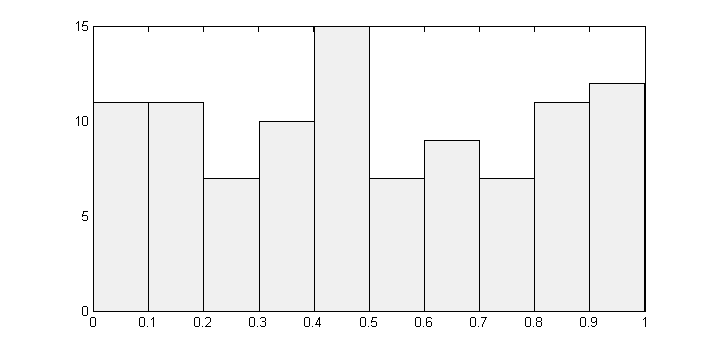
\includegraphics[width=5cm]{3AN}
   \inputminted[linenos,firstnumber=34,firstline=34,lastline=34]{matlab}{un.m}
   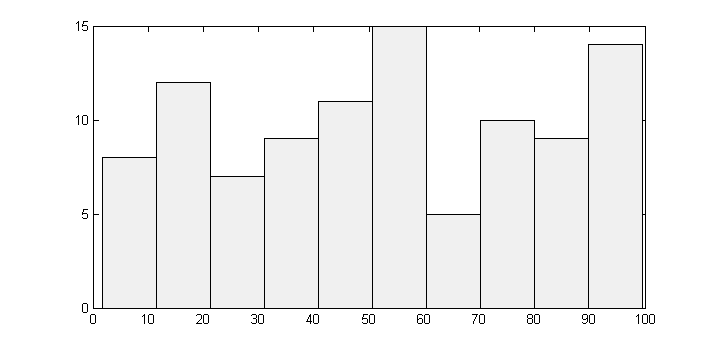
\includegraphics[width=5cm]{3AU}
  \subsection{}
   \inputminted[linenos,firstnumber=35,firstline=35,lastline=39]{matlab}{un.m}
  \subsection{}
   \inputminted[linenos,firstnumber=40,firstline=40,lastline=45]{matlab}{un.m}

 \section{Opérations sur les matrices}
  \inputminted[linenos,firstnumber=46,firstline=46,lastline=62]{matlab}{un.m}

 \section{Opérations sur les polynômes}
  \subsection{}
   \inputminted[linenos,firstnumber=63,firstline=63,lastline=66]{matlab}{un.m}

  \subsection{}
   \inputminted[linenos,firstnumber=67,firstline=67,lastline=69]{matlab}{un.m}

  \subsection{}
   \inputminted[linenos,firstnumber=70,firstline=70,lastline=72]{matlab}{un.m}

  \subsection{}
   \inputminted[linenos,firstnumber=73,firstline=73,lastline=75]{matlab}{un.m}

  \subsection{}
   \inputminted[linenos,firstnumber=76,firstline=76,lastline=80]{matlab}{un.m}

  \subsection{}
   \inputminted[linenos,firstnumber=81,firstline=81,lastline=82]{matlab}{un.m}

\end{document}
